
\documentclass[a4paper, 11pt, conference]{ieeeconf}  
                                                    
\overrideIEEEmargins
% See the \addtolength command later in the file to balance the column lengths
% on the last page of the document

\usepackage[utf8]{inputenc}
\usepackage{graphicx}
\usepackage{hyperref}
\usepackage{times} % assumes new font selection scheme installed
\usepackage{amsmath} % assumes amsmath package installed
\usepackage{amssymb}  % assumes amsmath package installed

\title{\LARGE \bf
Synchronous Stochastic Gradient Descent on Spark
}

\author{ \parbox{2 in}{\centering Jonathan Besomi \\
         {\tt\small jonathan.besomi@epfl.ch}}
         \parbox{2 in}{ \centering Yann Bolliger \\
        {\tt\small yann.bolliger@epfl.ch}}
        \parbox{2 in}{ \centering Kyle Gerard \\
        {\tt\small kyle.gerard@epfl.ch}}
}


\begin{document}



\maketitle
\thispagestyle{empty}
\pagestyle{plain}



\begin{abstract}
As part of a project for the course \textit{Systems for Data Science} we implemented a synchronous version of stochastic gradient descent (SGD) in Apache Spark (Scala), using Kubernetes as container orchestration. We compare our solution to an implementation from the previous year written in Python that supports synchronous and asynchronous communication. It results that our parallelised implementation with Spark yields better performance when more workers are involved. 
\end{abstract}

\section{INTRODUCTION}
The goal of this project is to implement synchronous SGD for a support vector machines (SVM) problem given in the Hogwild! paper \cite{hogwild-paper} and compare it against last year's project implementation \textit{hogwild-python} \cite{hogwild-python}. In order to fairly compare the two implementations we designed a solution that is similar to \cite{hogwild-python}.

Both implementations solve the same learning problem on the same data set (RCV1\footnote{Reuters Corpus Volume I. The data set used is an archive of over 800'000 manually categorised news-wire stories made available by Reuters.}). They also share the same loss function given below and they classify the same category of articles (``CCAT'').
$$
\mathcal{L}(\mathbf{w}) = 
\frac{1}{n} \sum_{i = 1}^{n} 
\max(0, 1- y_i(\mathbf{w}^\top \mathbf{x}_i - b))
+ \lambda \| \mathbf{w} \|^2
$$


\section{HOGWILD-PYTHON} 

We studied \cite{hogwild-python} with special attention given to the  synchronous case. As Spark is a purely synchronous computing framework we would not be able to build an asynchronous implementation with it. 

The results of \cite{hogwild-python} (Fig. \ref{their-figure}) show that while the program is very fast for few worker nodes (workers), the time to convergence increases with the number of workers! The report claims that the time to convergence is decreasing with the number of workers in the asynchronous case. However, it is visible from the second graph that the ``convergence'' happens at a higher loss. In order to get the same objective value even the asynchronous algorithm would need more time with more workers.

\begin{figure}[ht]
  \centering
  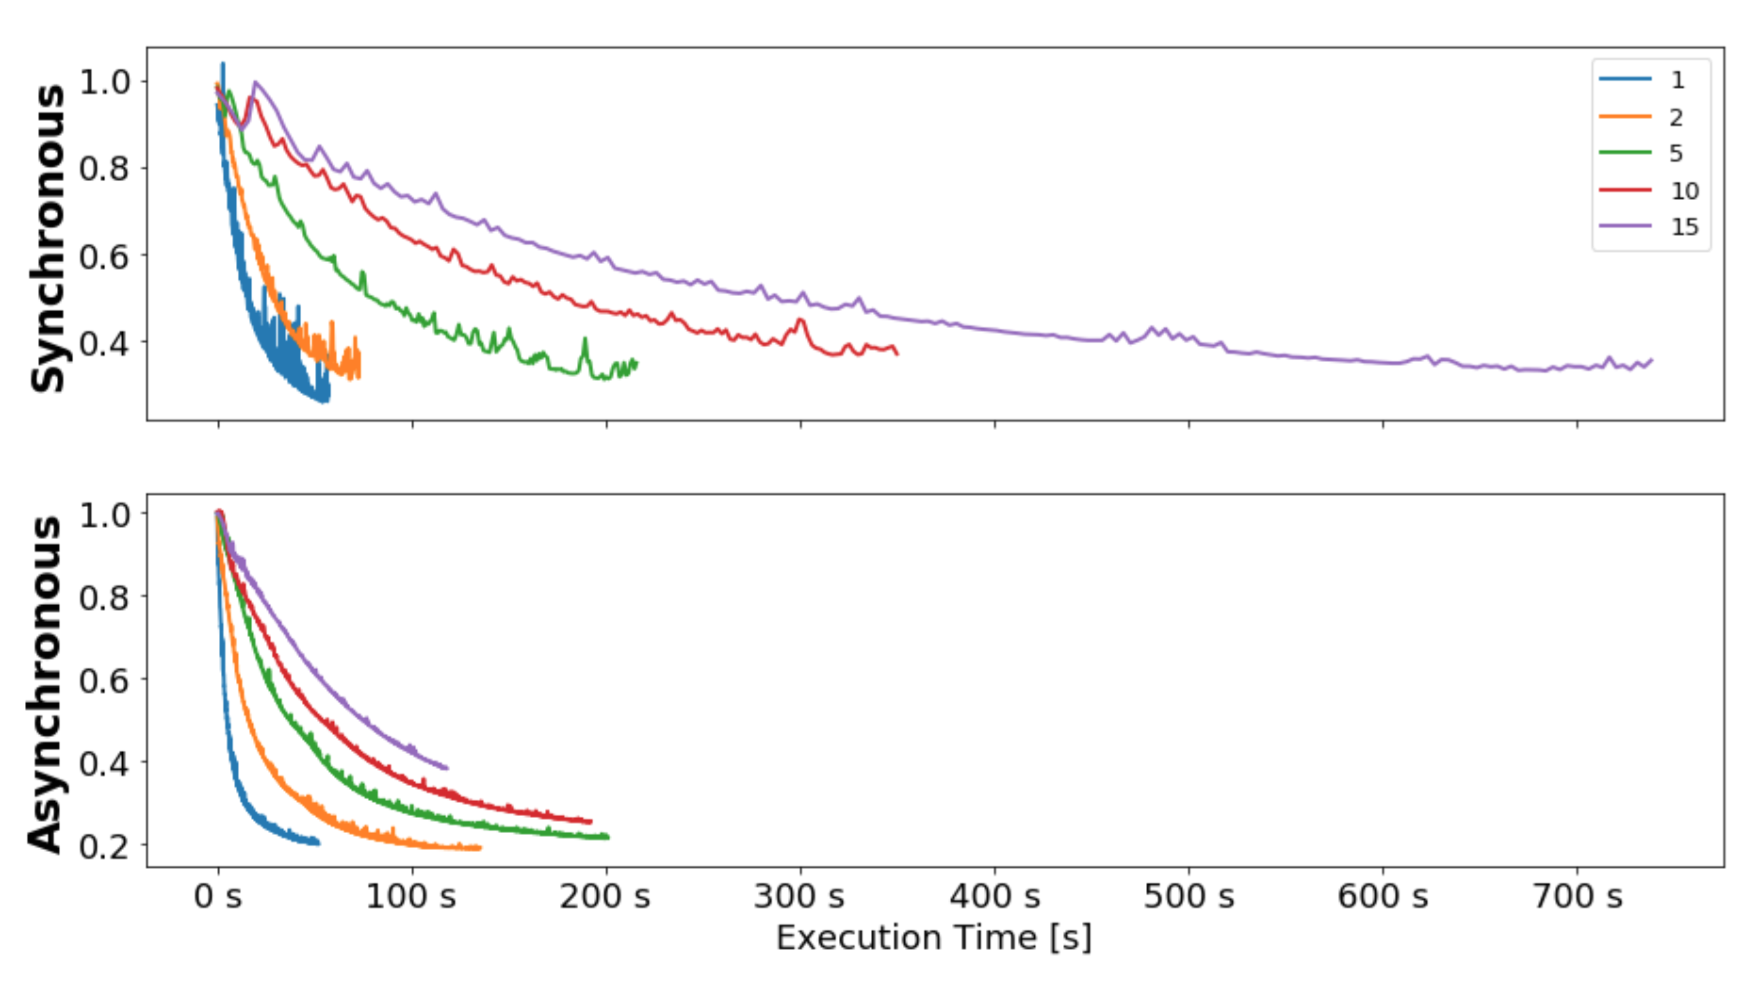
\includegraphics[scale=0.25]{their-figure-hogwild-python}
  \caption{Validation loss convergence of \textit{hogwild-python}. This figure is Fig. 4 from \cite{hogwild-python}.}
  \label{their-figure}
\end{figure}

This is counter-intuitive as one would expect the algorithm to converge more quickly with higher parallelism. 
We found two problems with \textit{hogwild-python}.

The first one is linked to the original idea of the Hogwild! algorithm \cite{hogwild-paper} that exploits the sparsity of the underlying problem. The assumption is that there are few collisions when workers concurrently update the weights and therefore the algorithm can still converge. \cite{hogwild-python} exploits this by updating the weights independently for each worker. Consequently, their learning rate is divided by the number of workers.
However, it seems that for more workers the learning rate gets too small and that more collisions occur. Both slow down the convergence -- as does the higher communication overhead. The latter is however not important for us because Spark also incurs this kind of overhead.

Secondly, as stated above, the implementation halts too early in some cases. This is due to the \textit{early stopping criterion} that simply checks whether the minimal loss in some window is increasing. To remedy this, we cloned the repository\footnote{\url{https://github.com/liabifano/hogwild-python}} and implemented a more patient, conservative stopping criterion (see \ref{implementation}). The same criterion is used for our Spark program in order to have comparable results.

\section{IMPLEMENTATION}
\label{implementation}

Our Spark implementation aims at improving both discussed problems.
Nonetheless, it tries to stay close to \textit{hogwild-python}. In particular, we output the same logging format, the programs can be run the same way from the command line and we use the same notebook for result analysis.

\subsection{Spark and weighted average}

\subsubsection{Data handling}

We use Spark RDDs as main data structure. That way all the data is automatically partitioned among the workers (executors in Spark) right from the initial read. To avoid shuffling, we partition the data points by their integer ID. A hash partitioner is used to create two partitions per executor. The \texttt{DataHelper} joins the labels and their vectors locally -- already leveraging the partitioning.

\subsubsection{Gradient calculation}
\label{gradient-calculation}

To exploit the sparsity of the input vectors we created a data type \texttt{SparseVector} that wraps a map storing only non-zero components of each vector.
By using only \texttt{mapValues} and \texttt{aggregate} in all data transformations of \texttt{SVM} we ensure that solely the weight vectors and the loss values will be communicated to the coordinator (driver in Spark). Because those are already accumulated locally by \texttt{aggregate}, the maximal communication payload is a single vector.
 
We introduce a new data type to tackle the problem of small learning rates and update collisions: \texttt{WeightedSparseVector}. As Spark's synchronicity makes independent updates of the weights impossible, we aggregate the weight updates of each sampled data point into a single vector before applying it. This allows for larger learning rates and sampling batches (subset sizes). But this also forces us to deal with collisions: In a test one component was updated more than 100 times more than another component of the weights.

The solution is to take a weighted average over all the stochastic updates. Our data structure automatically keeps count of how many data points update a component. In the end, it returns a weighted stochastic gradient. This also solves the problem that the number of samples per batch on each partition might differ.

\subsubsection{Loss calculation}
Contrary to \cite{hogwild-python} we calculate the validation loss in the same distributed fashion as the gradients. This is because the data already is in a partitioned RDD and therefore it is natural to aggregate the loss in that way. 

\subsubsection{Learning rate}
As stated above, our learning rate is not divided by the number of workers. It is given by $0.3 \max(1, \min(3, \frac{\beta}{500}))$, where $\beta$ is the total batch size over all workers. Hence, the rate slightly increases for larger batch sizes. This is possible because larger batches are less noisy due to averaging.


\subsubsection{Stopping criterion}

Our stopping criterion takes two equally long windows (20 epochs) and checks whether the average validation losses satisfy:
$$
l_{old} - l_{new} < \epsilon 
$$
If this is the case, the algorithm stops. The criterion is less sensitive to fluctuation and therefore we don't halt too early.

\subsection{Kubernetes and Deploy}

Spark provides a bash script to submit jobs to Kubernetes, \texttt{spark-submit.sh}. It requires a Docker image that will be loaded and executed on different machines (workers). The Docker image is pulled by Kubernetes from Docker Hub. 

The \texttt{docker-image-tool.sh}, another bash script of Spark, is used to build and push the image to the public registry. Without using caching, the build and push of the image takes multiple minutes. In order to speed up the build process, we prefer to cache all build steps of the Dockerfile except the copying of the JAR. To circumvent caching when building the JAR, we assign a unique name to the JAR file. That way, during the build process at the step when the JAR file is copied into the image, the filename is not recognised and a fresh version of the JAR file is loaded.

The main script used to deploy and execute the code is \texttt{run.sh}\footnote{For a detailed description of the different parameters accepted, please refer to the \texttt{README} in the root of our code repository.}. It follows these steps to successfully execute a job on Kubernetes:
\begin{enumerate}
	\item If Spark does not exist on the local machine, download it in a folder inside the deploy folder called \texttt{spark}
	\item Build the JAR file, append a random unique string to the filename
	\item Construct the Dockerfile, loading the JAR into the image
	\item Build and push the Docker image on Docker Hub
	\item \texttt{spark-submit} the job to Kubernetes
\end{enumerate}

Once the job is done, a log file is saved on the \textit{persistent volume}. Another bash script \texttt{download-log.sh} temporarily creates a new pod linked to our persistent volume, downloads all the log files of all the experiments and ultimately deletes the pod. This solution differs from the one implemented by \cite{hogwild-python} since we don't continuously check if the log file exists and download it before Kubernetes terminates. Instead, we start a new pod and download all the files at once.

\section{EXPERIMENTS}

In order to find out which of the three implementations produces the best-quality result in the shortest amount of time, we do not closely study the accuracy of each trained model. Indeed, all three implementations use the same algorithm and thus reach the same optimal values with similar parameters (learning rate, regression lambda) given enough time. 

Instead, the goal of this paper is to understand the differences in the time it takes for each implementation to converge to an optimal validation loss. Our main metric will be validation loss as a function of training time. More precisely, we measure the time it takes to reach a goal validation loss of 0.25. We will not be using training time i.e. time to the halting of the algorithm as a metric (as was used in \cite{hogwild-python}). Indeed, we do not find this metric to be reliable enough considering how difficult it is to stop the training upon convergence in a similar manner for all implementations (synchronous/asynchronous).

We will evaluate how each implementation performs as a function of the number of workers available $n$ and of the subset size $s$. The subset size is the subset of data points given to each worker to calculate the stochastic gradient in distributed manner. For the Spark implementation for example, this means that at each iteration, $s \cdot n$ samples are evaluated. For each implementation we test all combinations of the following parameters:
$$
(n, s) \in \{1, 5, 10, 20\} \times \{50, 100, 1000\}
$$
The ideal implementation will converge for all configurations and will be faster as the number of workers increases.


\addtolength{\textheight}{-1.6cm}   

% This command serves to balance the column lengths
% on the last page of the document manually. It shortens
% the textheight of the last page by a suitable amount.
% This command does not take effect until the next page
% so it should come on the page before the last. Make
% sure that you do not shorten the textheight too much.


\section{RESULTS} 

\begin{table}[t]
\caption{Best accuracy reached for each implementation}
\begin{tabular}{|l|l|l|l|}
\hline
Implementation & Best params & Train Acc. & Valid Acc. \\ \hline
\textit{hogwild-python} sync & w=1, s=100 & 0.95 & 0.94 \\ \hline
\textit{hogwild-python} async & \textbf{w=1, s=100} & 0.95 & 0.94 \\ \hline
Spark sync & w=10, s=100 & 0.97 & 0.94 \\ \hline
\end{tabular}
\label{accuracy}
\end{table}


\begin{figure}[t]
  \centering
  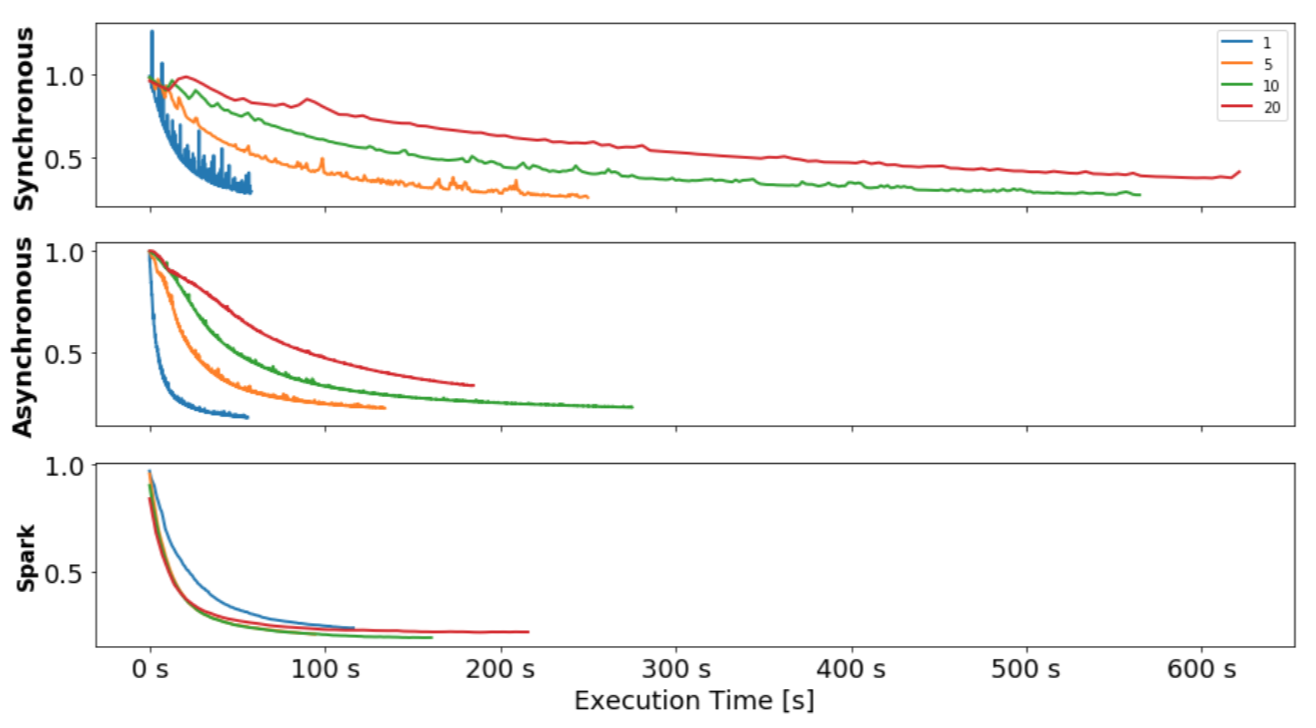
\includegraphics[scale=0.36]{worker-count.png}
  \caption{Validation loss as a function of training time, number of workers with subset size 100.}
  \label{workercount}
\end{figure}


As expected, we can see from Table \ref{accuracy} that the validation accuracy reached by all three implementations is the same. Thus, given enough time, all implementations provide the same quality of results.


\subsection{Number of workers}

From Figure \ref{workercount} we see that all three implementations converge in a similar manner with a single worker. However, as the number of workers increases, the Spark implementation converges faster whereas both Python implementations become much slower.
This difference is central in answering our paper's main question. Indeed, as workers are added, our Spark implementation is not overwhelmed by the added communication overhead and thus, the convergence continues to increase in speed. 

On the other hand, both Python implementations incur problems as the number of workers increases. Indeed, their rate of validation loss convergence is dramatically reduced. This means that the benefit of adding workers (and making more processing power available to calculate gradients) is not worth the increase in communication overhead. For this reason, our synchronous Spark implementation is more efficient and more useful in its task to distribute the machine learning workload across multiple workers. Therefore, as soon as there is more than a single worker, our Spark implementation can be considered as faster than the \textit{hogwild-python} implementations.




\subsection{Subset size per worker}
As predicted in section II, the convergence of the validation loss for \cite{hogwild-python} gets slower as the number of workers is increased. However, both implementations (synchronous and asynchronous) have similar convergence of the validation loss with different subset sizes. We can see this in Figure \ref{subsetpy}.

Similarly for Spark, Figure \ref{subsetspark} shows that for all subset sizes the time to convergence is relatively similar as a function of the number of workers. This means that our Spark implementation is also robust to different configurations of subset sizes.


\begin{figure}[ht]
  \centering
  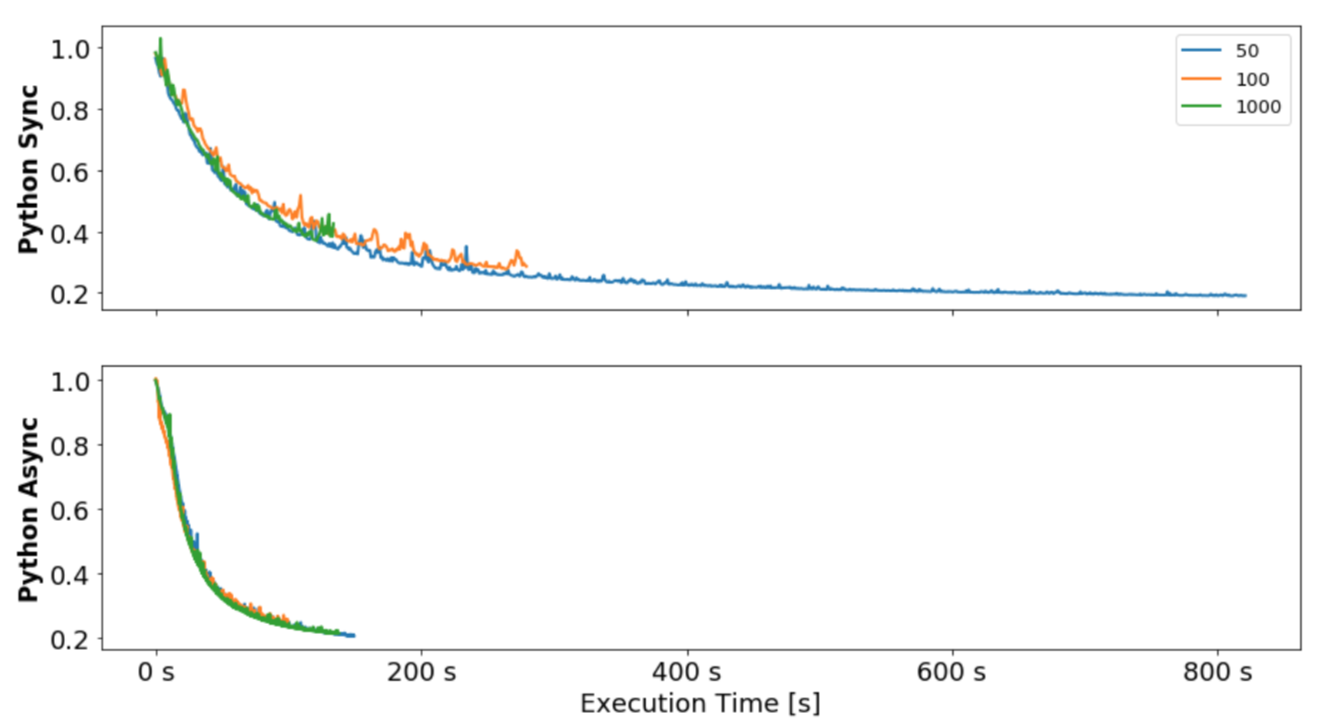
\includegraphics[scale=0.35]{subsetpy.png}
  \caption{Validation loss as a function of training time and subset sizes $\{50, 100, 1000\}$ for \textit{hogwild-python} implementations, with a fixed number of workers (5).}
  \label{subsetpy}
\end{figure}

\begin{figure}[ht]
  \centering
  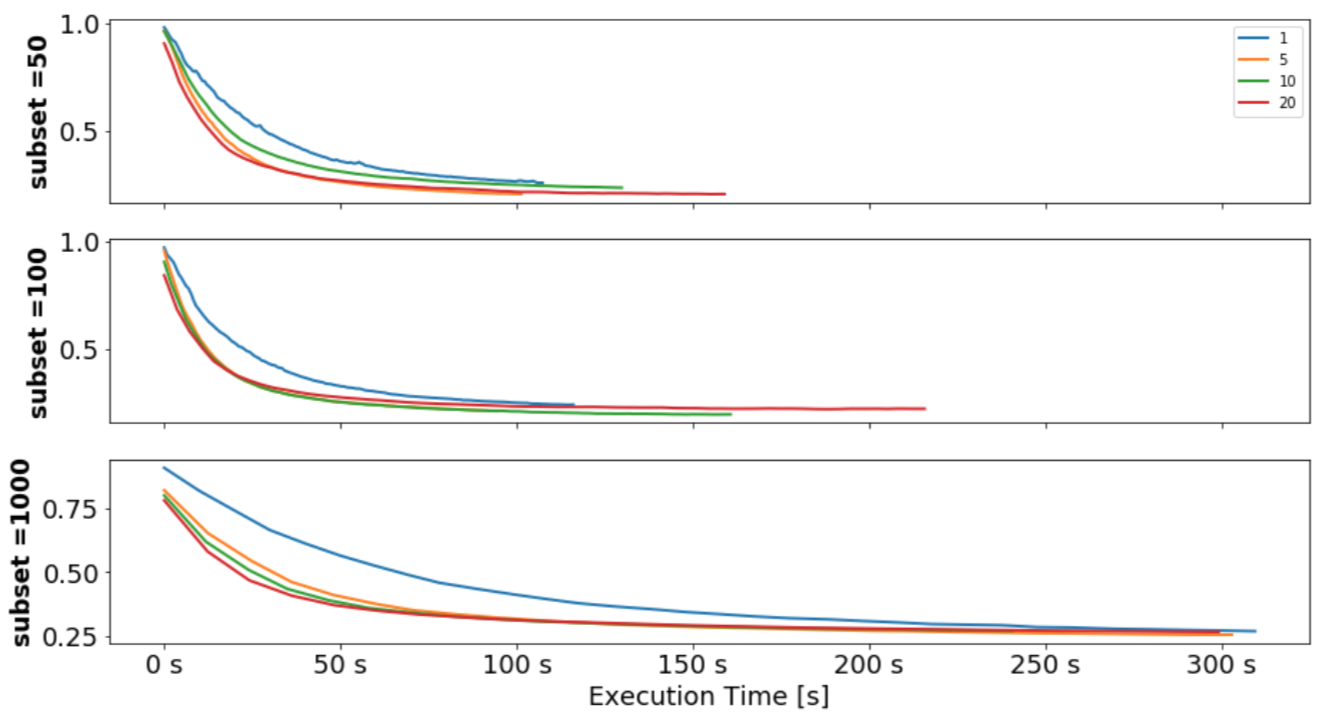
\includegraphics[scale=0.35]{spark-subset.png}
  \caption{Validation loss as a function of training time, number of workers  $\{1, 5, 10, 20\}$ and subset size for our Spark implementation.}
  \label{subsetspark}
\end{figure}


\subsection{Additional observations}
We also remark that in both Figure \ref{workercount} and Figure \ref{subsetspark} the validation loss of the Spark implementation is a lot smoother than for the Python implementations. This is due to our weighted average solution described in section \ref{gradient-calculation}.

Table \ref{valloss} shows that the fastest convergence to the objective validation loss of 0.25 is reached with a single worker for the asynchronous Python implementation. The reason for this is due to a relatively small training set size (only 23149 samples) which means that a single process is sufficient for this task and can load all the samples into its memory. We do not expect this to be true with a much larger training set.


\begin{table}[ht]
\caption{Time to reach validation loss of 0.25 for each implementation}
\begin{tabular}{|l|l|l|}
\hline
Implementation & Best params & Time to val. loss 0.25 \\ \hline
\textit{hogwild-python}  sync & w=1, s=100 & 82.6 seconds \\ \hline
\textit{hogwild-python}  async & \textbf{w=1, s=100} & 54.3 seconds \\ \hline
Spark sync & w=10, s=50 & 80.1 seconds \\ \hline
\end{tabular}
\label{valloss}
\end{table}


\section{CONCLUSIONS}

In this paper we compared the \textit{hogwild-python} asynchronous and synchronous implementations to our synchronous Spark implementation. The \textit{hogwild-python} project was very ambitious due to the complexity of not only having to distribute the SGD algorithm but also having to take care of the communication between workers and the coordinator. Our Spark implementation is less complex owing to Spark taking care of communication between nodes.

However, we found some limitations to the Hogwild! solution \cite{hogwild-paper}. It is the need to decrease the learning rate when increasing the number of workers because of the necessity of sparse weight updates as the group explained in their report: ``If we did not adapt the learning rate to the subset size, we are running into the risk of the loss not converging.'' \cite[p. 4]{hogwild-python}.

The solution we introduced in our Spark implementation to overcome this limitation was the use of weighted averaging when aggregating the stochastic gradients at each iteration. There is no risk of divergence and moreover, this solution could be added to the synchronous version of \textit{hogwild-python}.

\thispagestyle{empty}



\section*{ACKNOWLEDGMENT}

We thank the \textit{hogwild-python} team from last year.


\begin{thebibliography}{99} 

\bibitem{hogwild-paper} Benjamin; Re Christopher; Wright Stephen J. Niu, Feng; Recht. Hogwild!: A lock-free approach to parallelizing stochastic gradient descent. eprint arXiv:1106.5730, 2011.

\bibitem{hogwild-python} L. Bifano, R. Bachmann and M. Allemann, Distributed asynchronous SGD, EPFL, unpublished, 2018.

\end{thebibliography}

\end{document}